\section{Nonlinear Regression}
\subsection{Prior Works}
\begin{frame}{Approximation Method}
  \begin{itemize}
    \item 2nd Order Volterra Kernel \cite{Friston2000}
    \note{Quadratic Approximation}
    \begin{itemize}
        \item Quadratic Convolution used to approximate Jacobian Matrix.
        \note{Because of the nonlinearities in the BOLD model, step size for
                integrating would otherwise be extremely small}
        \item Volterra approximation quality is not known.
    \end{itemize}
    \note{Volterra Approximation depends on sparsity etc}
    {\footnotesize
    $$y(t) = k_0 + \int_{-\infty}^{\infty} k_1(s_1) x(t-s_1) ds_1
        + \int_{-\infty}^{\infty} k_2(s_1,s_2) x(t-s_1)x(t-s_2) ds_1 ds_2$$
        \note{Its possible this isn't even knowable}
    }
    \item Canonical Hemodynamic Response Function
    \note{Linear Approximation}
    \begin{itemize}
        \item No Parameters Estimated
        \item Maximum Likelihood Possible
        \item Inflexible - even to changes in onset time
    \end{itemize}
    \begin{center}
    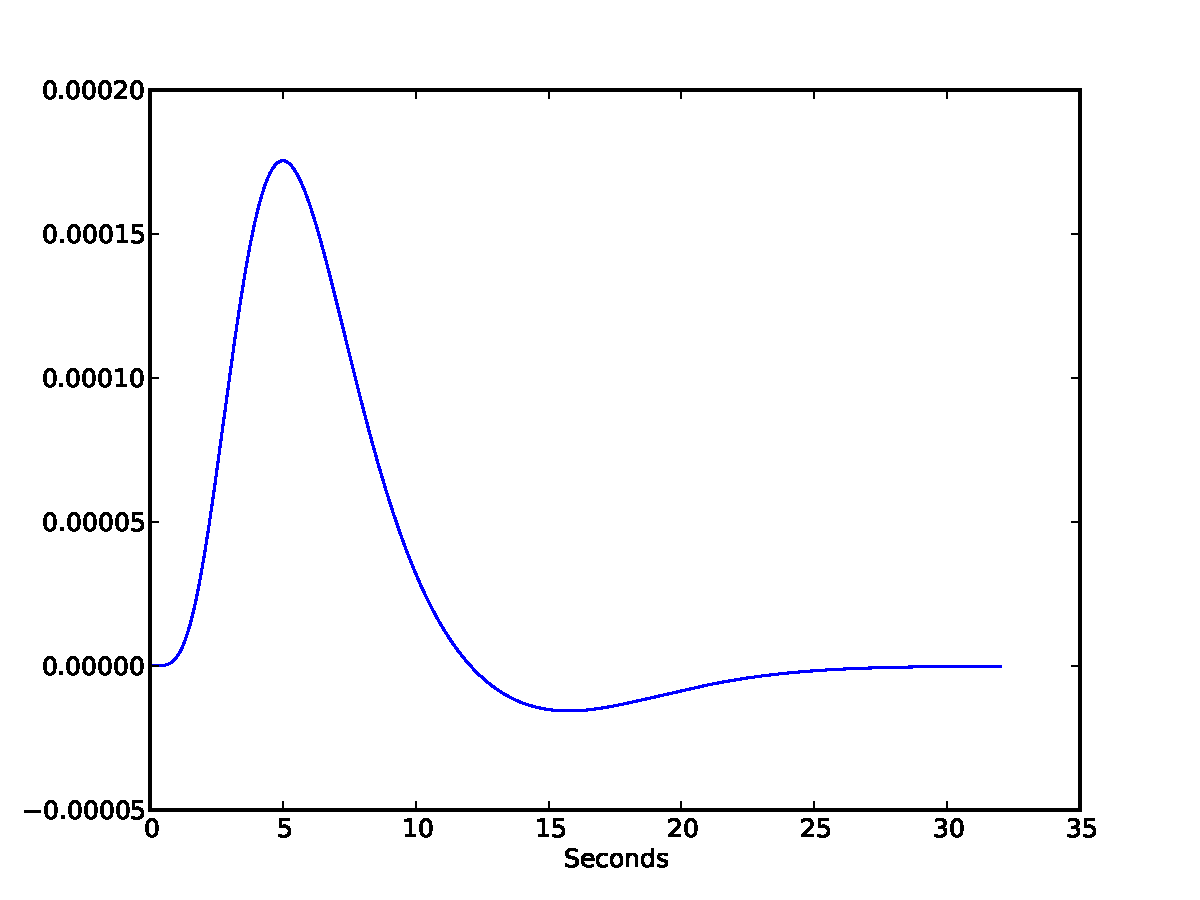
\includegraphics[clip=true,trim=4.88cm 0cm 5cm 1.5cm,height=2.7cm,width=8cm]{HRF}
    \end{center}
    
  \end{itemize}
\end{frame}

\begin{frame}{Nonlinear Methods}
\begin{itemize}
    \begin{columns}
    \begin{column}{.42\textwidth}
    \item Local Linearization filter, \cite{Riera2003}
    $$f(t)- f(t-1) \sim N(0, \sigma^2)$$
     \note{Jacobian of the $\dot{x}$ is available, making gradient descent possible}
    \item Genetic Algorithms and Simulated Annealing, \cite{Vakorin2007}
     \note{Genetic Algorithms were used to optimize spike points, simulated annealing for the parameters}
    \item Particle Filters to estimate States, \cite{Murray2009}
    \begin{itemize}
        \item ML estimate of $\Theta$, \cite{Johnston2007}
         \note{Particle Filter used to estimate states, ML of parameters based on the posterior of states and so on}
    \end{itemize}
    \item Unscented Kalman Filter \cite{Hu2009}
     \note{Technically Kalman Filters and Particle Filters are Bayesian Filters}
     \note{Essentially filtering out inconsistent parameters.}
    \end{column}

    \begin{column}{.58\textwidth}
    \begin{figure}
    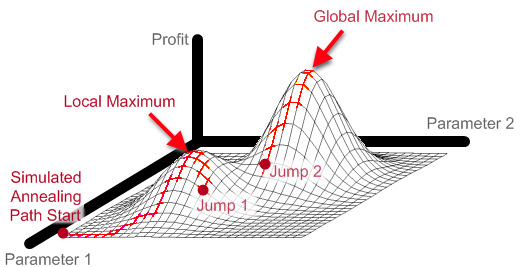
\includegraphics[clip=true,trim=0cm 0cm 0cm 1cm,width=.6\textwidth]{simulated_annealing}
    \caption{Simulated Annealing can escape local minima with chaotic jumps. \cite{Dama}}
    \end{figure}
    \begin{figure}
    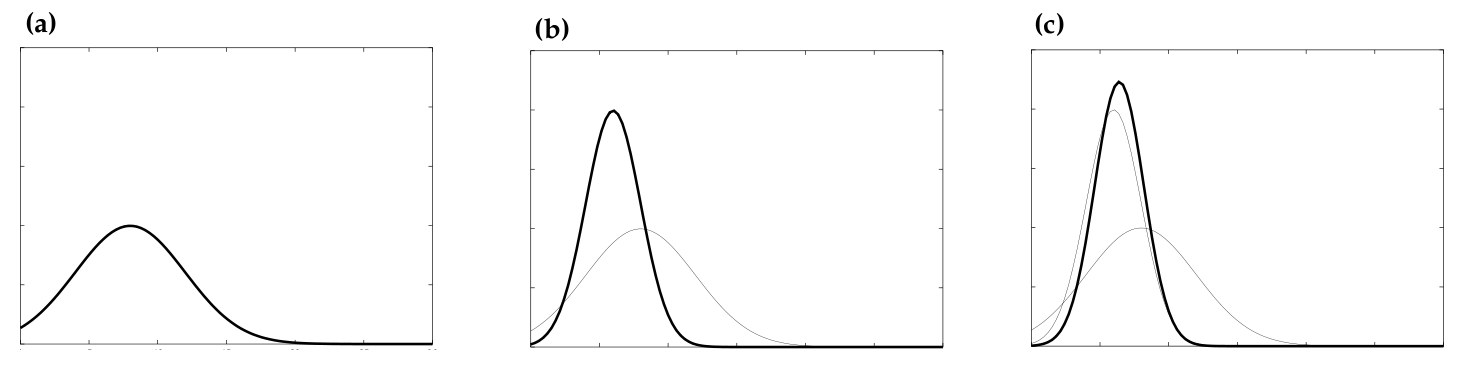
\includegraphics[width=\textwidth]{kalman}
    \caption{UKF: (a) Initial Belief  (b) Noisy Measurement  (c) incorporated into the belief. \cite{Thrun2005}}
    \end{figure}
    \end{column}
    \end{columns}
\end{itemize}
\end{frame}

\subsection{Particle Filter}
%frame with example
\begin{frame}{Example System Identification}
\begin{itemize}
\item Given:
    \begin{itemize}
    \item Elevation Map (1D)
    \item Ability To Measure Elevation
    \end{itemize}
\item Particle Consists of the unknowns:
    \begin{itemize}
    \item State: Location  $[0, 20]$
    \item Constant: Direction  $\{Left, Right\}$
    \end{itemize}
\end{itemize}

\begin{center}
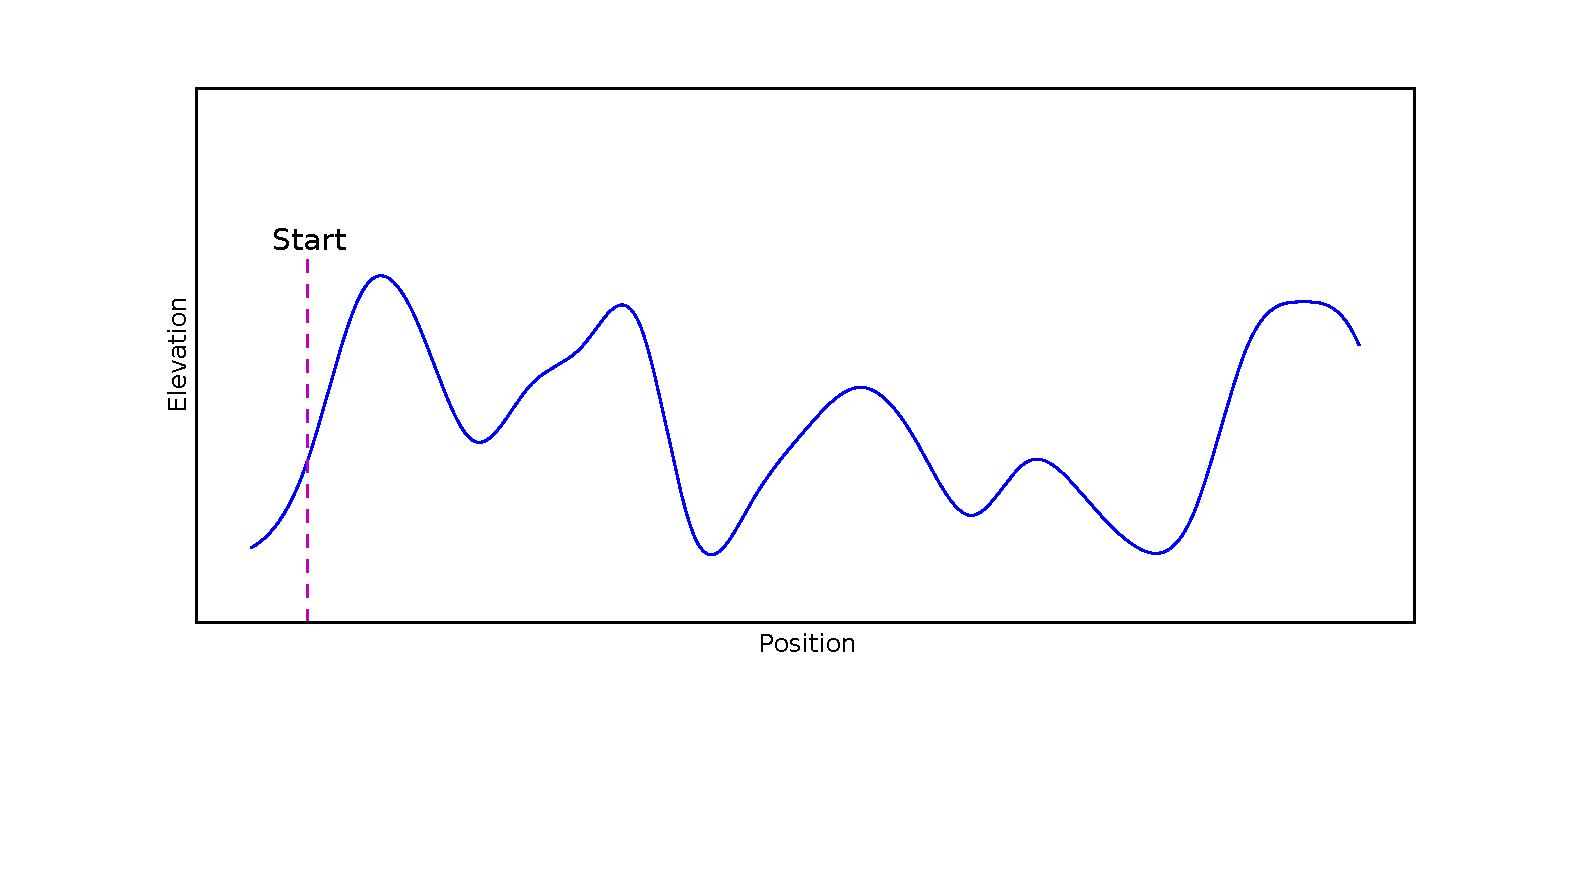
\includegraphics[clip=true,trim=2cm 3cm 3cm 3cm,width=.7\textwidth]{setup}
\end{center}
\end{frame}

\begin{frame}{Initial Distribution}
\centering
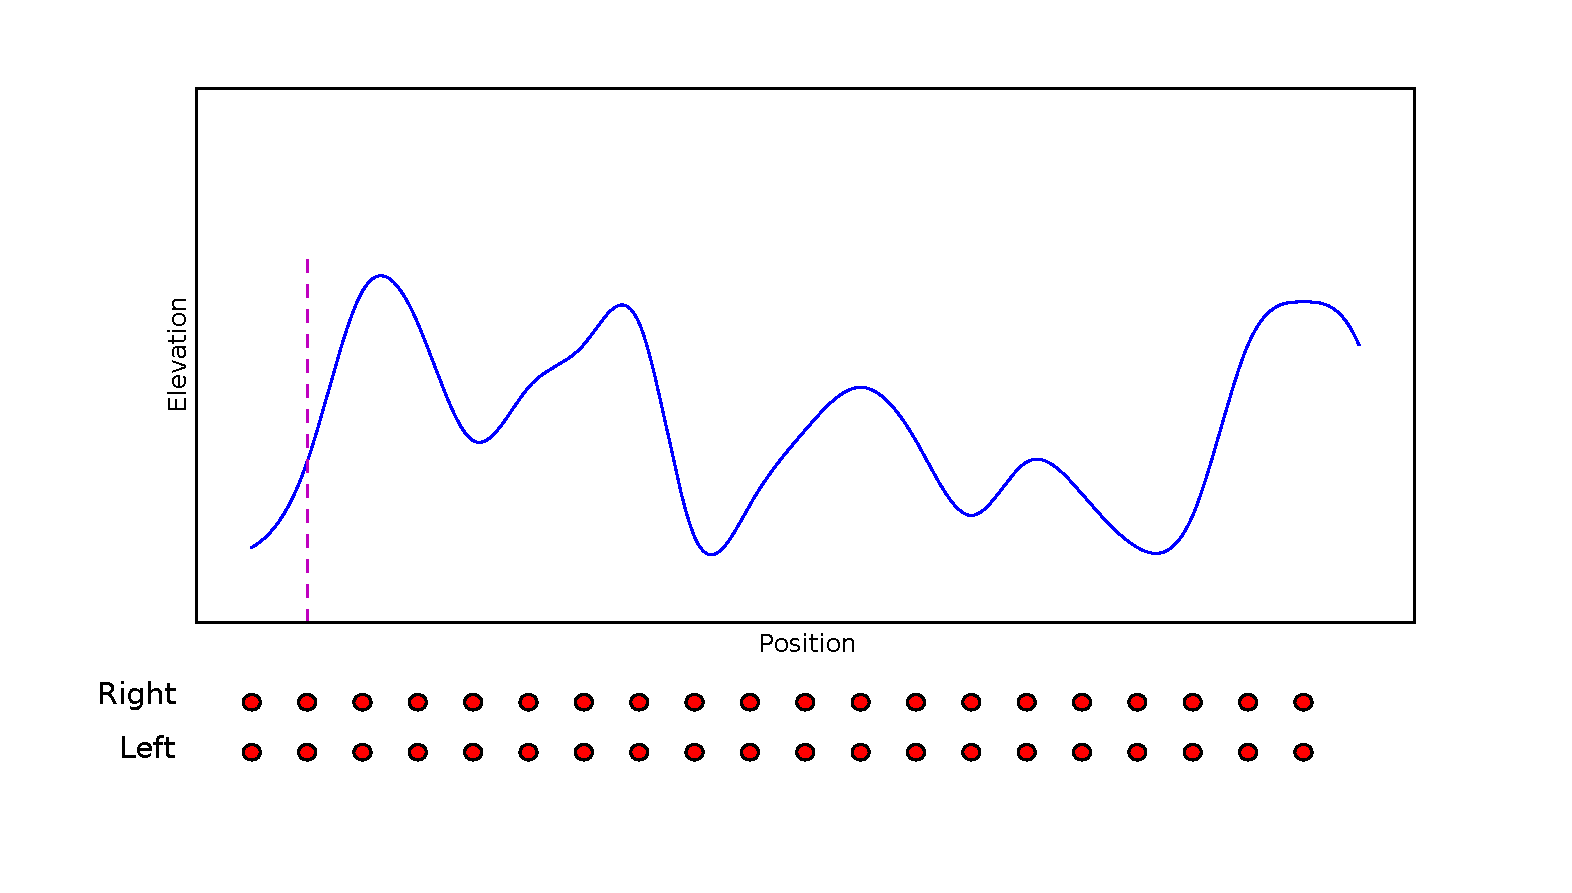
\includegraphics[width=\textwidth]{init}\\
\end{frame}

\begin{frame}{Measurement 1}
\centering
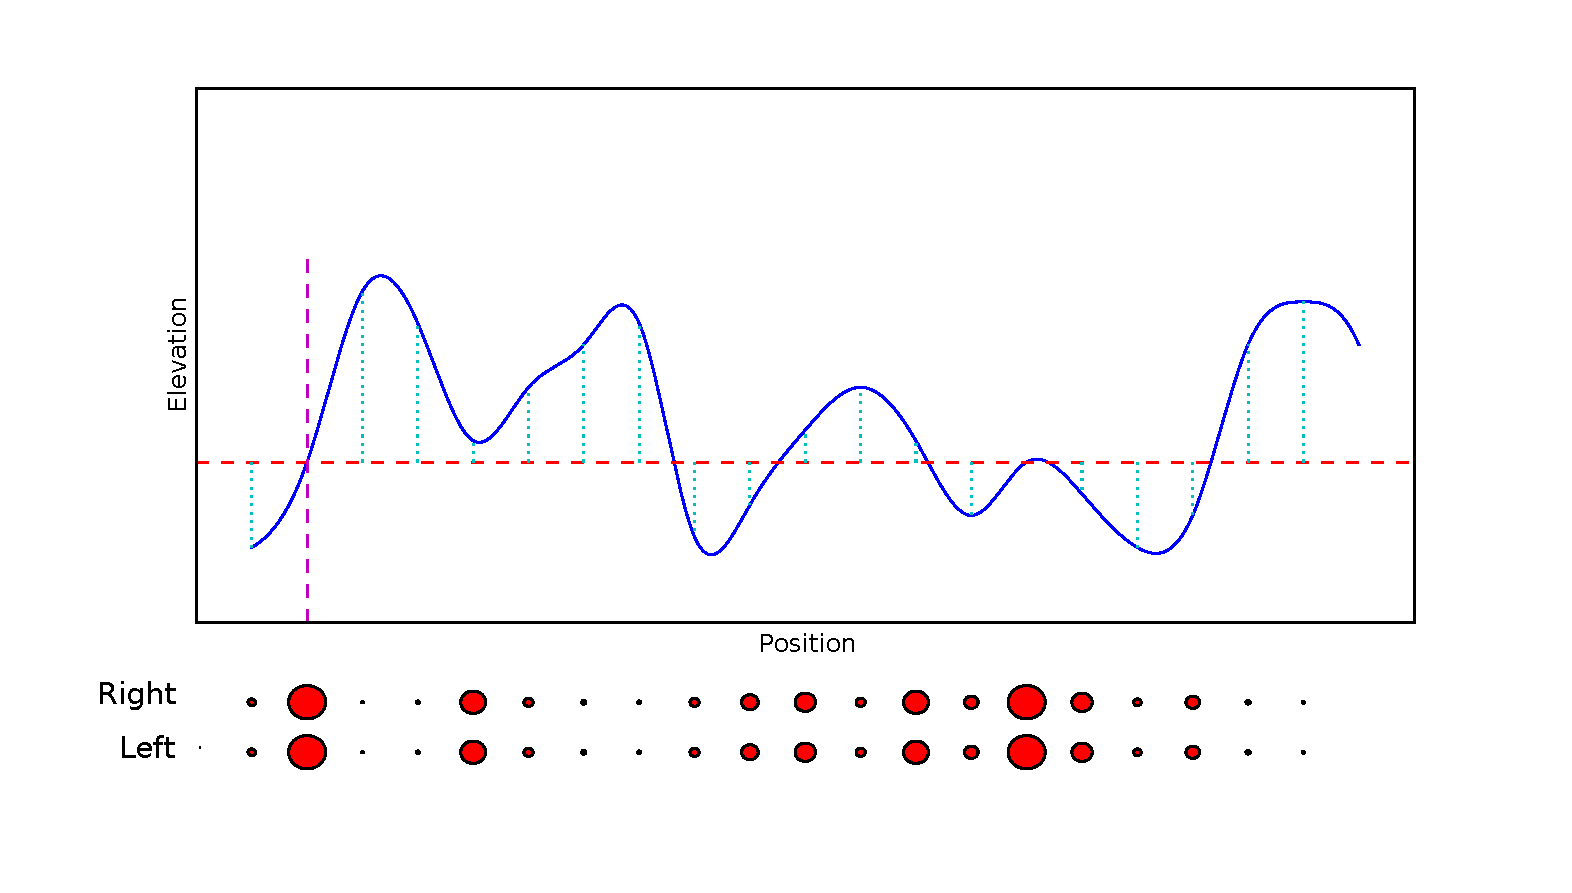
\includegraphics[width=\textwidth]{meas1}\\
\end{frame}

\begin{frame}{Step Forward}
\centering
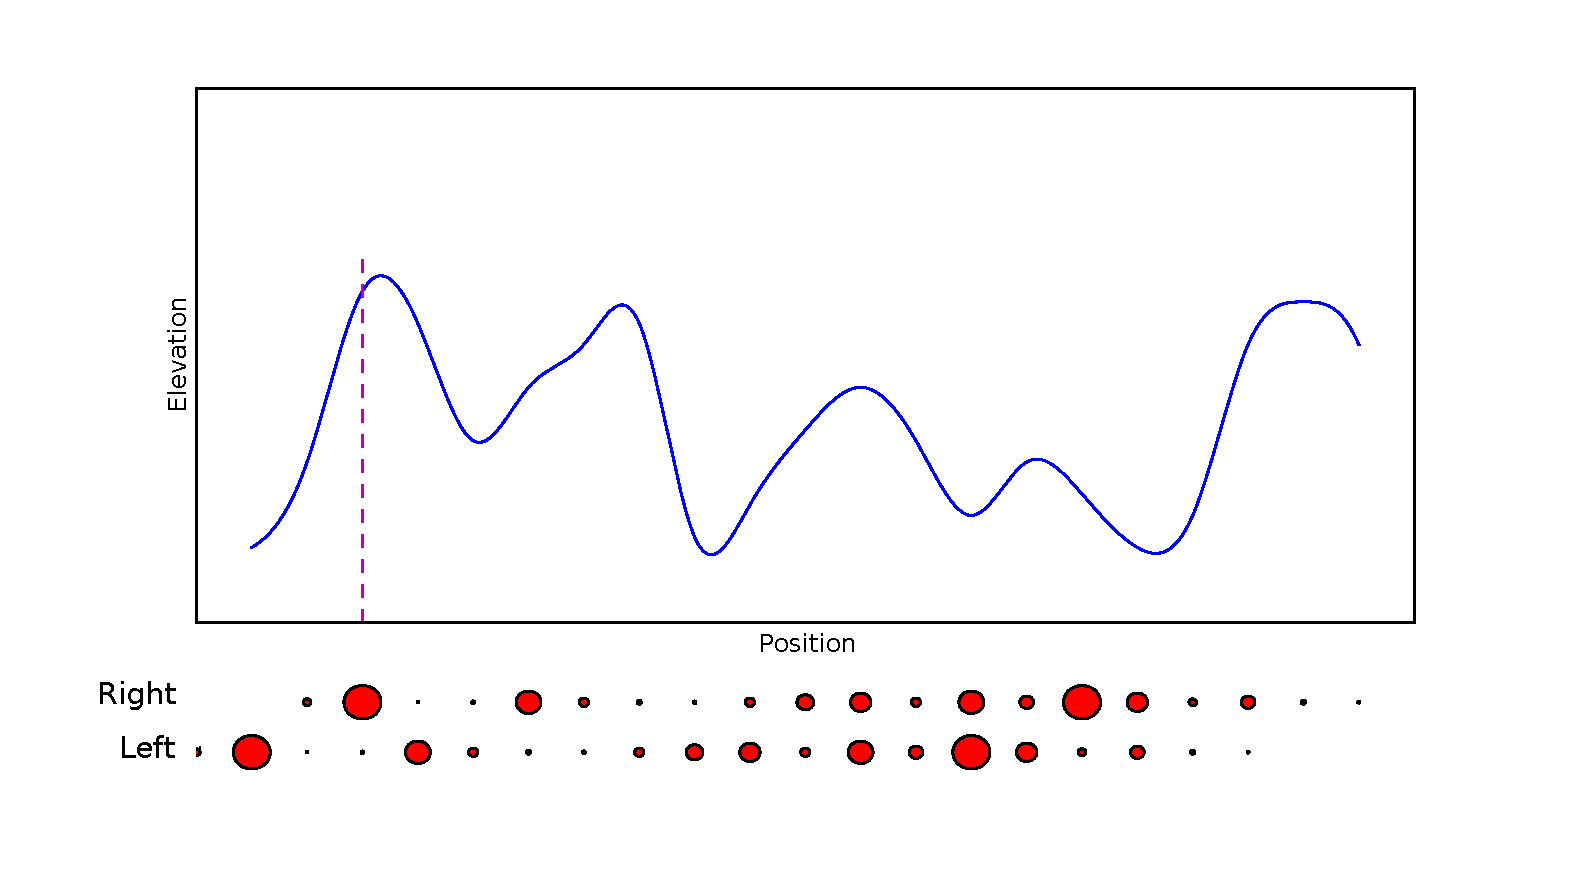
\includegraphics[width=\textwidth]{move1}\\
\end{frame}

\begin{frame}{Measurement 2}
\centering
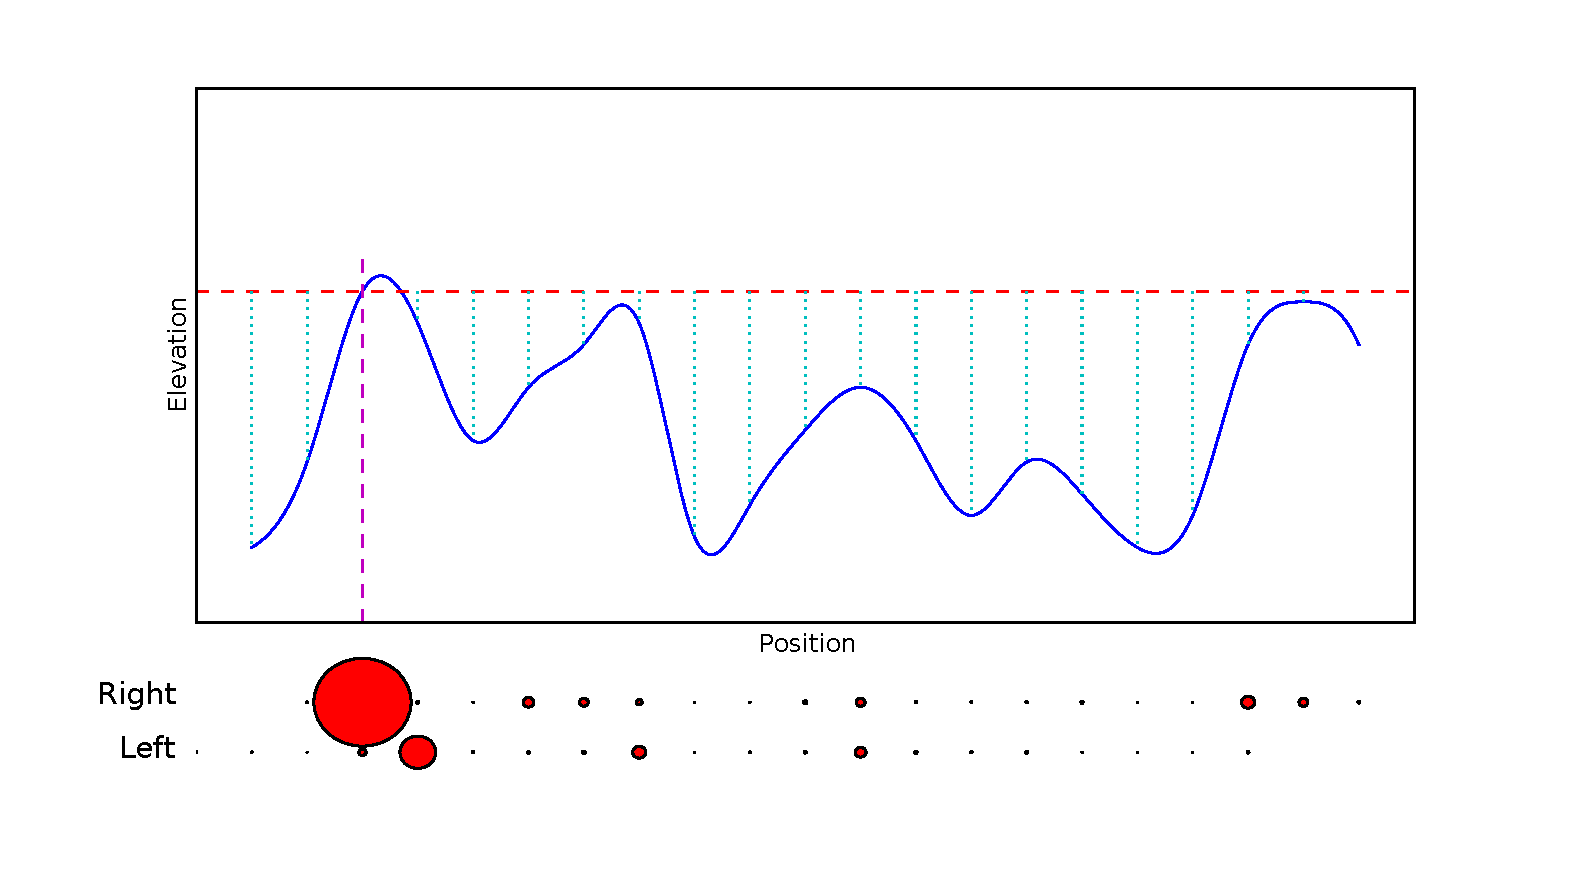
\includegraphics[width=\textwidth]{meas2}\\
\end{frame}

\begin{frame}{Step Forward}
\centering
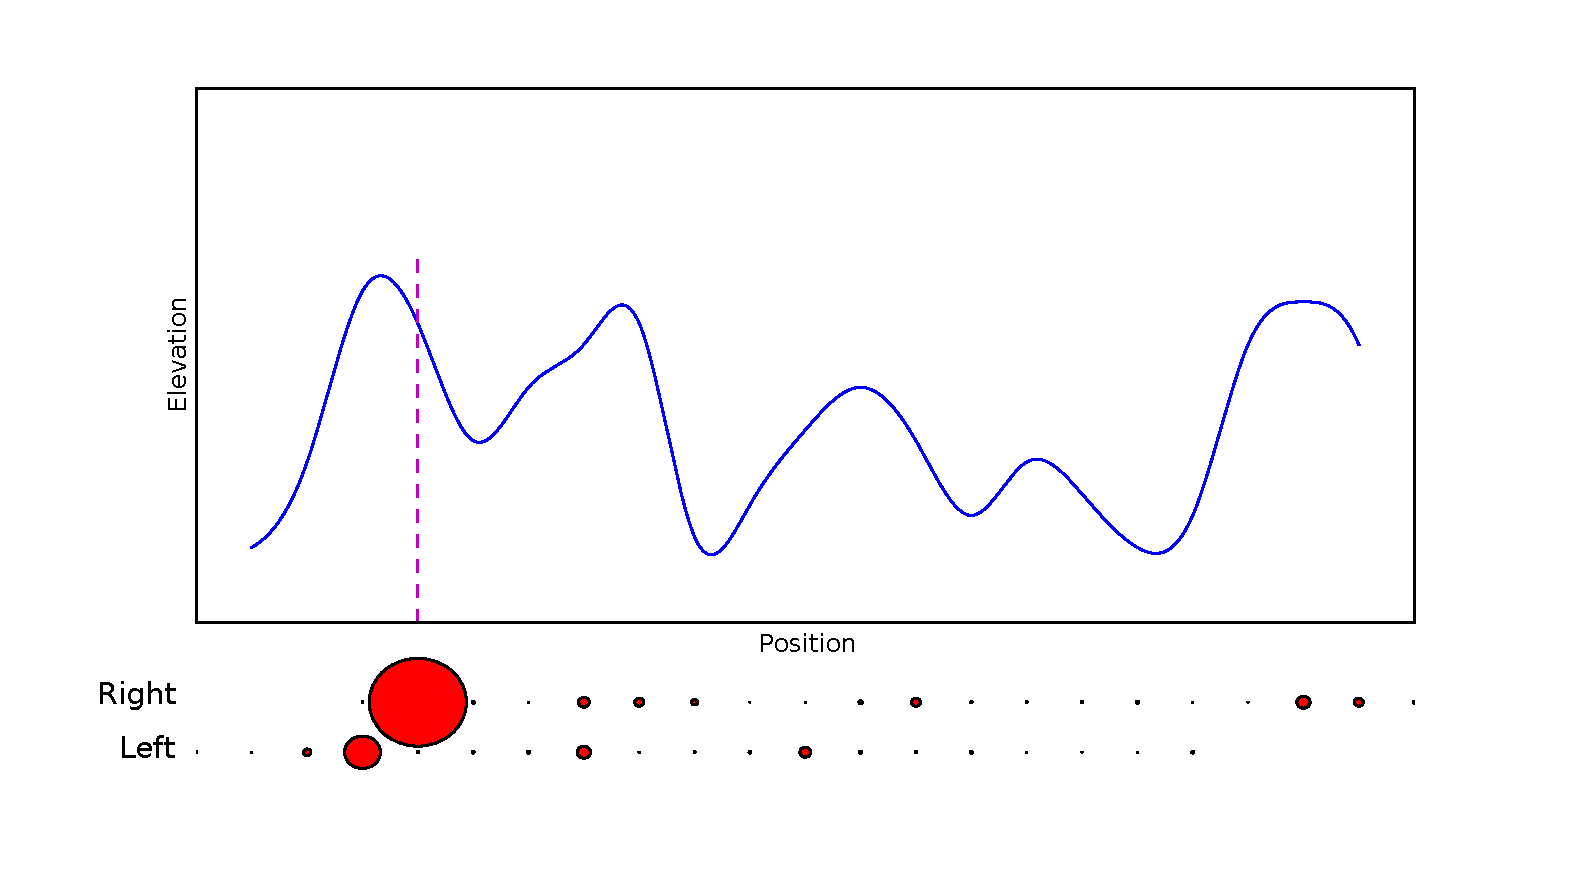
\includegraphics[width=\textwidth]{move2}\\
\end{frame}

\begin{frame}{Particle Filter Concepts}
\small
\begin{columns}
\begin{column}{.5\textwidth}
\begin{itemize}
    \item Weighting Function
        \begin{itemize}
            \item Converts Discrete Estimates of $y$ 
                    Into a Continuous Estimate of $y$
        \end{itemize}
    \item Resampling
    \begin{itemize}
        \item Remove Useless Particles
    \end{itemize}
    \item Regularized Resampling
    \begin{itemize}
        \item Prevent Identical Particles
    \end{itemize}
\end{itemize}
\end{column}

\begin{column}{.5\textwidth}
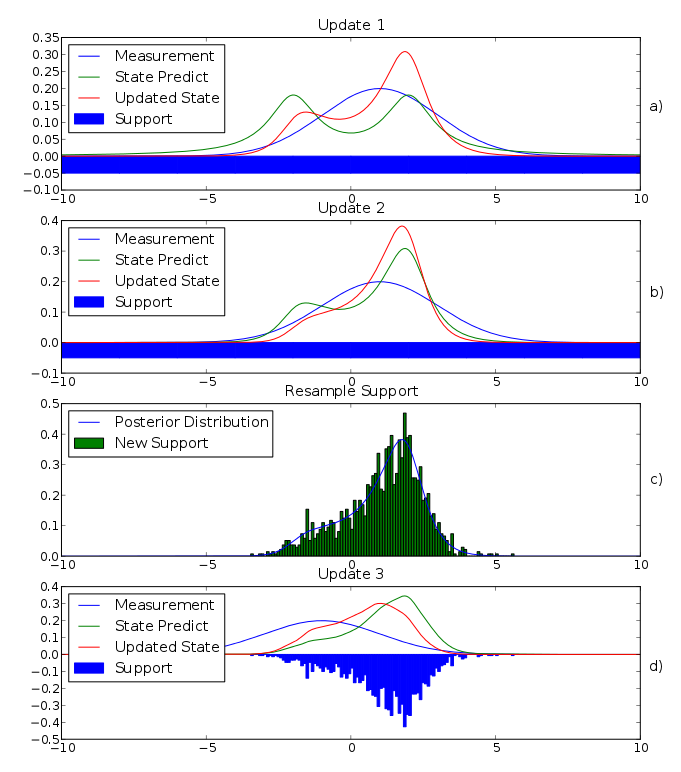
\includegraphics[clip=true,trim=.75cm 7.07cm .5cm 7cm,width=\textwidth]{particle_filter2}
\end{column}
\end{columns}
\end{frame}

\begin{frame}{Particle Construction, Particle $i$, Time $k$}
\begin{columns}
\begin{column}{.54\textwidth}
\begin{itemize}
    \item Mixture PDF, with $N_p$ particles:
        $$P(x_k) = \sum_{i=0}^{N_p} w^i\delta(x_k - x^i_k ) dx$$
    \item Weight Definition:
        $$w^i_k \propto \frac{P(x^i_{0:k} | y_{0:k})}{q(x^i_{0:k} | y_{0:k})}$$
      \note{$q$ is the density/location of the particle}
      \note{$p$ is the actual probability }
    \item Incorporating Measurement $y_k$:
        $$w^i_k \propto & w^i_{k-1}P(y_k| x_k) $$
      \note{Because of the proportion, note that the weights do not
            have to integrate to 1, and can be extremely large or extremely small}
\end{itemize}
\end{column}

\begin{column}{.46\textwidth}
\tiny
\ifx\du\undefined
  \newlength{\du}
\fi
\setlength{\du}{10\unitlength}
\begin{tikzpicture}
\pgftransformxscale{1.000000}
\pgftransformyscale{-1.000000}
\definecolor{dialinecolor}{rgb}{0.000000, 0.000000, 0.000000}
\pgfsetstrokecolor{dialinecolor}
\definecolor{dialinecolor}{rgb}{1.000000, 1.000000, 1.000000}
\pgfsetfillcolor{dialinecolor}
\pgfsetlinewidth{0.050000\du}
\pgfsetdash{}{0pt}
\definecolor{dialinecolor}{rgb}{1.000000, 1.000000, 1.000000}
\pgfsetfillcolor{dialinecolor}
\fill (9.250000\du,3.650000\du)--(9.250000\du,5.050000\du)--(12.1000\du,5.050000\du)--(12.1000\du,3.650000\du)--cycle;
\definecolor{dialinecolor}{rgb}{0.000000, 0.000000, 0.000000}
\pgfsetstrokecolor{dialinecolor}
\draw (9.250000\du,3.650000\du)--(9.250000\du,5.050000\du)--(12.1000\du,5.050000\du)--(12.1000\du,3.650000\du)--cycle;
% setfont left to latex
\definecolor{dialinecolor}{rgb}{0.000000, 0.000000, 0.000000}
\pgfsetstrokecolor{dialinecolor}
\node at (10.732500\du,4.600000\du){Particle};
\definecolor{dialinecolor}{rgb}{1.000000, 1.000000, 1.000000}
\pgfsetfillcolor{dialinecolor}
\fill (9.250000\du,5.050000\du)--(9.250000\du,14.050000\du)--(12.1000\du,14.050000\du)--(12.1000\du,5.050000\du)--cycle;
\definecolor{dialinecolor}{rgb}{0.000000, 0.000000, 0.000000}
\pgfsetstrokecolor{dialinecolor}
\draw (9.250000\du,5.050000\du)--(9.250000\du,14.050000\du)--(12.1000\du,14.050000\du)--(12.1000\du,5.050000\du)--cycle;
% setfont left to latex
\definecolor{dialinecolor}{rgb}{0.000000, 0.000000, 0.000000}
\pgfsetstrokecolor{dialinecolor}
\node[anchor=west] at (9.400000\du,5.750000\du){\color{mblue} $s$};
% setfont left to latex
\definecolor{dialinecolor}{rgb}{0.000000, 0.000000, 0.000000}
\pgfsetstrokecolor{dialinecolor}
\node[anchor=west] at (9.400000\du,6.550000\du){\color{mblue} $f$};
% setfont left to latex
\definecolor{dialinecolor}{rgb}{0.000000, 0.000000, 0.000000}
\pgfsetstrokecolor{dialinecolor}
\node[anchor=west] at (9.400000\du,7.350000\du){\color{mblue} $q$};
% setfont left to latex
\definecolor{dialinecolor}{rgb}{0.000000, 0.000000, 0.000000}
\pgfsetstrokecolor{dialinecolor}
\node[anchor=west] at (9.400000\du,8.150000\du){\color{mblue} $v$};
% setfont left to latex
\definecolor{dialinecolor}{rgb}{0.000000, 0.000000, 0.000000}
\pgfsetstrokecolor{dialinecolor}
\node[anchor=west] at (9.400000\du,8.950000\du){\color{mred} $\epsilon$};
% setfont left to latex
\definecolor{dialinecolor}{rgb}{0.000000, 0.000000, 0.000000}
\pgfsetstrokecolor{dialinecolor}
\node[anchor=west] at (9.400000\du,9.750000\du){\color{mred} $\tau_f$};
% setfont left to latex
\definecolor{dialinecolor}{rgb}{0.000000, 0.000000, 0.000000}
\pgfsetstrokecolor{dialinecolor}
\node[anchor=west] at (9.400000\du,10.550000\du){\color{mred} $\tau_s$};
% setfont left to latex
\definecolor{dialinecolor}{rgb}{0.000000, 0.000000, 0.000000}
\pgfsetstrokecolor{dialinecolor}
\node[anchor=west] at (9.400000\du,11.350000\du){\color{mred} $\tau_0$};
% setfont left to latex
\definecolor{dialinecolor}{rgb}{0.000000, 0.000000, 0.000000}
\pgfsetstrokecolor{dialinecolor}
\node[anchor=west] at (9.400000\du,12.150000\du){\color{mred} $\alpha$};
% setfont left to latex
\definecolor{dialinecolor}{rgb}{0.000000, 0.000000, 0.000000}
\pgfsetstrokecolor{dialinecolor}
\node[anchor=west] at (9.400000\du,12.950000\du){\color{mred} $E_0$};
% setfont left to latex
\definecolor{dialinecolor}{rgb}{0.000000, 0.000000, 0.000000}
\pgfsetstrokecolor{dialinecolor}
\node[anchor=west] at (9.400000\du,13.750000\du){\color{mred} $V_0$};
\definecolor{dialinecolor}{rgb}{1.000000, 1.000000, 1.000000}
\pgfsetfillcolor{dialinecolor}
\fill (9.250000\du,14.050000\du)--(9.250000\du,15.050000\du)--(12.1000\du,15.050000\du)--(12.1000\du,14.050000\du)--cycle;
\definecolor{dialinecolor}{rgb}{0.000000, 0.000000, 0.000000}
\pgfsetstrokecolor{dialinecolor}
\draw (9.250000\du,14.050000\du)--(9.250000\du,15.050000\du)--(12.1000\du,15.050000\du)--(12.1000\du,14.050000\du)--cycle;
% setfont left to latex
\definecolor{dialinecolor}{rgb}{0.000000, 0.000000, 0.000000}
\pgfsetstrokecolor{dialinecolor}
\node[anchor=west] at (9.400000\du,14.750000\du){ weight};
% setfont left to latex
\definecolor{dialinecolor}{rgb}{0.000000, 0.000000, 0.000000}
\pgfsetstrokecolor{dialinecolor}
\node[anchor=west] at (5.050000\du,5.850000\du){};
% setfont left to latex
\definecolor{dialinecolor}{rgb}{0.000000, 0.000000, 0.000000}
\pgfsetstrokecolor{dialinecolor}
\node[anchor=west] at (5.100000\du,6.500000\du){Change};
% setfont left to latex
\definecolor{dialinecolor}{rgb}{0.000000, 0.000000, 0.000000}
\pgfsetstrokecolor{dialinecolor}
\node[anchor=west] at (5.100000\du,7.300000\du){With Time};
% setfont left to latex
\definecolor{dialinecolor}{rgb}{0.000000, 0.000000, 0.000000}
\pgfsetstrokecolor{dialinecolor}
\node[anchor=west] at (13.000000\du,9.850000\du){Change When};
% setfont left to latex
\definecolor{dialinecolor}{rgb}{0.000000, 0.000000, 0.000000}
\pgfsetstrokecolor{dialinecolor}
\node[anchor=west] at (13.000000\du,10.650000\du){Resampling};
\pgfsetlinewidth{0.050000\du}
\pgfsetdash{}{0pt}
\pgfsetdash{}{0pt}
\pgfsetbuttcap
{
\definecolor{dialinecolor}{rgb}{0.000000, 0.000000, 0.000000}
\pgfsetfillcolor{dialinecolor}
% was here!!!
\definecolor{dialinecolor}{rgb}{0.000000, 0.000000, 0.000000}
\pgfsetstrokecolor{dialinecolor}
\pgfpathmoveto{\pgfpoint{9.000025\du}{5.399967\du}}
\pgfpatharc{217}{144}{1.000000\du and 1.000000\du}
\pgfusepath{stroke}
}
\pgfsetlinewidth{0.050000\du}
\pgfsetdash{}{0pt}
\pgfsetdash{}{0pt}
\pgfsetbuttcap
{
\definecolor{dialinecolor}{rgb}{0.000000, 0.000000, 0.000000}
\pgfsetfillcolor{dialinecolor}
% was here!!!
\definecolor{dialinecolor}{rgb}{0.000000, 0.000000, 0.000000}
\pgfsetstrokecolor{dialinecolor}
\pgfpathmoveto{\pgfpoint{9.000025\du}{6.999967\du}}
\pgfpatharc{217}{144}{1.000000\du and 1.000000\du}
\pgfusepath{stroke}
}
\pgfsetlinewidth{0.050000\du}
\pgfsetdash{}{0pt}
\pgfsetdash{}{0pt}
\pgfsetbuttcap
{
\definecolor{dialinecolor}{rgb}{0.000000, 0.000000, 0.000000}
\pgfsetfillcolor{dialinecolor}
% was here!!!
\definecolor{dialinecolor}{rgb}{0.000000, 0.000000, 0.000000}
\pgfsetstrokecolor{dialinecolor}
\draw (9.000000\du,6.600000\du)--(8.600000\du,6.800000\du);
}
\pgfsetlinewidth{0.050000\du}
\pgfsetdash{}{0pt}
\pgfsetdash{}{0pt}
\pgfsetbuttcap
{
\definecolor{dialinecolor}{rgb}{0.000000, 0.000000, 0.000000}
\pgfsetfillcolor{dialinecolor}
% was here!!!
\definecolor{dialinecolor}{rgb}{0.000000, 0.000000, 0.000000}
\pgfsetstrokecolor{dialinecolor}
\draw (8.600000\du,6.800000\du)--(9.000000\du,7.000000\du);
}
\pgfsetlinewidth{0.050000\du}
\pgfsetdash{}{0pt}
\pgfsetdash{}{0pt}
\pgfsetbuttcap
{
\definecolor{dialinecolor}{rgb}{0.000000, 0.000000, 0.000000}
\pgfsetfillcolor{dialinecolor}
% was here!!!
\definecolor{dialinecolor}{rgb}{0.000000, 0.000000, 0.000000}
\pgfsetstrokecolor{dialinecolor}
\pgfpathmoveto{\pgfpoint{12.399753\du}{9.80\du}}
\pgfpatharc{10}{-9}{12.965299\du and 12.965299\du}
\pgfusepath{stroke}
}
\pgfsetlinewidth{0.050000\du}
\pgfsetdash{}{0pt}
\pgfsetdash{}{0pt}
\pgfsetbuttcap
{
\definecolor{dialinecolor}{rgb}{0.000000, 0.000000, 0.000000}
\pgfsetfillcolor{dialinecolor}
% was here!!!
\definecolor{dialinecolor}{rgb}{0.000000, 0.000000, 0.000000}
\pgfsetstrokecolor{dialinecolor}
\pgfpathmoveto{\pgfpoint{12.419203\du}{15.0\du}}
\pgfpatharc{10}{-9}{12.847799\du and 12.847799\du}
\pgfusepath{stroke}
}
\pgfsetlinewidth{0.050000\du}
\pgfsetdash{}{0pt}
\pgfsetdash{}{0pt}
\pgfsetbuttcap
{
\definecolor{dialinecolor}{rgb}{0.000000, 0.000000, 0.000000}
\pgfsetfillcolor{dialinecolor}
% was here!!!
\definecolor{dialinecolor}{rgb}{0.000000, 0.000000, 0.000000}
\pgfsetstrokecolor{dialinecolor}
\draw (12.400000\du,9.800000\du)--(13.019438\du,10.220000\du);
}
\pgfsetlinewidth{0.050000\du}
\pgfsetdash{}{0pt}
\pgfsetdash{}{0pt}
\pgfsetbuttcap
{
\definecolor{dialinecolor}{rgb}{0.000000, 0.000000, 0.000000}
\pgfsetfillcolor{dialinecolor}
% was here!!!
\definecolor{dialinecolor}{rgb}{0.000000, 0.000000, 0.000000}
\pgfsetstrokecolor{dialinecolor}
\draw (13.019438\du,10.220000\du)--(12.440000\du,10.760000\du);
}
% setfont left to latex
\definecolor{dialinecolor}{rgb}{0.000000, 0.000000, 0.000000}
\pgfsetstrokecolor{dialinecolor}
\node[anchor=west] at (4.000000\du,15.000000\du){Change When};
% setfont left to latex
\definecolor{dialinecolor}{rgb}{0.000000, 0.000000, 0.000000}
\pgfsetstrokecolor{dialinecolor}
\node[anchor=west] at (4.000000\du,15.800000\du){Incorporating Measurement};
\pgfsetlinewidth{0.050000\du}
\pgfsetdash{}{0pt}
\pgfsetdash{}{0pt}
\pgfsetbuttcap
{
\definecolor{dialinecolor}{rgb}{0.000000, 0.000000, 0.000000}
\pgfsetfillcolor{dialinecolor}
% was here!!!
\definecolor{dialinecolor}{rgb}{0.000000, 0.000000, 0.000000}
\pgfsetstrokecolor{dialinecolor}
\draw (9.000000\du,14.200000\du)--(8.600000\du,14.800000\du);
}
\pgfsetlinewidth{0.050000\du}
\pgfsetdash{}{0pt}
\pgfsetdash{}{0pt}
\pgfsetbuttcap
{
\definecolor{dialinecolor}{rgb}{0.000000, 0.000000, 0.000000}
\pgfsetfillcolor{dialinecolor}
% was here!!!
\definecolor{dialinecolor}{rgb}{0.000000, 0.000000, 0.000000}
\pgfsetstrokecolor{dialinecolor}
\draw (9.000000\du,15.000000\du)--(8.600000\du,14.800000\du);
}
\end{tikzpicture}

\end{column}
\end{columns}
\end{frame}

%\ifx\du\undefined
%  \newlength{\du}
%\fi
%\setlength{\du}{10\unitlength}
%\begin{tikzpicture}
%\pgftransformxscale{1.000000}
%\pgftransformyscale{-1.000000}
%\definecolor{dialinecolor}{rgb}{0.000000, 0.000000, 0.000000}
%\pgfsetstrokecolor{dialinecolor}
%\definecolor{dialinecolor}{rgb}{1.000000, 1.000000, 1.000000}
%\pgfsetfillcolor{dialinecolor}
%\pgfsetlinewidth{0.050000\du}
%\pgfsetdash{}{0pt}
%\definecolor{dialinecolor}{rgb}{1.000000, 1.000000, 1.000000}
%\pgfsetfillcolor{dialinecolor}
%\fill (9.250000\du,3.650000\du)--(9.250000\du,5.050000\du)--(13.215000\du,5.050000\du)--(13.215000\du,3.650000\du)--cycle;
%\definecolor{dialinecolor}{rgb}{0.000000, 0.000000, 0.000000}
%\pgfsetstrokecolor{dialinecolor}
%\draw (9.250000\du,3.650000\du)--(9.250000\du,5.050000\du)--(13.215000\du,5.050000\du)--(13.215000\du,3.650000\du)--cycle;
%% setfont left to latex
%\definecolor{dialinecolor}{rgb}{0.000000, 0.000000, 0.000000}
%\pgfsetstrokecolor{dialinecolor}
%\node at (11.232500\du,4.600000\du){Particle};
%\definecolor{dialinecolor}{rgb}{1.000000, 1.000000, 1.000000}
%\pgfsetfillcolor{dialinecolor}
%\fill (9.250000\du,5.050000\du)--(9.250000\du,14.050000\du)--(13.215000\du,14.050000\du)--(13.215000\du,5.050000\du)--cycle;
%\definecolor{dialinecolor}{rgb}{0.000000, 0.000000, 0.000000}
%\pgfsetstrokecolor{dialinecolor}
%\draw (9.250000\du,5.050000\du)--(9.250000\du,14.050000\du)--(13.215000\du,14.050000\du)--(13.215000\du,5.050000\du)--cycle;
%% setfont left to latex
%\definecolor{dialinecolor}{rgb}{0.000000, 0.000000, 0.000000}
%\pgfsetstrokecolor{dialinecolor}
%\node[anchor=west] at (9.400000\du,5.750000\du){\color{mblue} $s$};
%% setfont left to latex
%\definecolor{dialinecolor}{rgb}{0.000000, 0.000000, 0.000000}
%\pgfsetstrokecolor{dialinecolor}
%\node[anchor=west] at (9.400000\du,6.550000\du){\color{mblue} $f$};
%% setfont left to latex
%\definecolor{dialinecolor}{rgb}{0.000000, 0.000000, 0.000000}
%\pgfsetstrokecolor{dialinecolor}
%\node[anchor=west] at (9.400000\du,7.350000\du){\color{mblue} $q$};
%% setfont left to latex
%\definecolor{dialinecolor}{rgb}{0.000000, 0.000000, 0.000000}
%\pgfsetstrokecolor{dialinecolor}
%\node[anchor=west] at (9.400000\du,8.150000\du){\color{mblue} $v$};
%% setfont left to latex
%\definecolor{dialinecolor}{rgb}{0.000000, 0.000000, 0.000000}
%\pgfsetstrokecolor{dialinecolor}
%\node[anchor=west] at (9.400000\du,8.950000\du){\color{mred} $\epsilon$};
%% setfont left to latex
%\definecolor{dialinecolor}{rgb}{0.000000, 0.000000, 0.000000}
%\pgfsetstrokecolor{dialinecolor}
%\node[anchor=west] at (9.400000\du,9.750000\du){\color{mred} $\tau_f$};
%% setfont left to latex
%\definecolor{dialinecolor}{rgb}{0.000000, 0.000000, 0.000000}
%\pgfsetstrokecolor{dialinecolor}
%\node[anchor=west] at (9.400000\du,10.550000\du){\color{mred} $\tau_s$};
%% setfont left to latex
%\definecolor{dialinecolor}{rgb}{0.000000, 0.000000, 0.000000}
%\pgfsetstrokecolor{dialinecolor}
%\node[anchor=west] at (9.400000\du,11.350000\du){\color{mred} $\tau_0$};
%% setfont left to latex
%\definecolor{dialinecolor}{rgb}{0.000000, 0.000000, 0.000000}
%\pgfsetstrokecolor{dialinecolor}
%\node[anchor=west] at (9.400000\du,12.150000\du){\color{mred} $\alpha$};
%% setfont left to latex
%\definecolor{dialinecolor}{rgb}{0.000000, 0.000000, 0.000000}
%\pgfsetstrokecolor{dialinecolor}
%\node[anchor=west] at (9.400000\du,12.950000\du){\color{mred} $\E_0$};
%% setfont left to latex
%\definecolor{dialinecolor}{rgb}{0.000000, 0.000000, 0.000000}
%\pgfsetstrokecolor{dialinecolor}
%\node[anchor=west] at (9.400000\du,13.750000\du){\color{mred} $V_0$};
%\definecolor{dialinecolor}{rgb}{1.000000, 1.000000, 1.000000}
%\pgfsetfillcolor{dialinecolor}
%\fill (9.250000\du,14.050000\du)--(9.250000\du,15.050000\du)--(13.215000\du,15.050000\du)--(13.215000\du,14.050000\du)--cycle;
%\definecolor{dialinecolor}{rgb}{0.000000, 0.000000, 0.000000}
%\pgfsetstrokecolor{dialinecolor}
%\draw (9.250000\du,14.050000\du)--(9.250000\du,15.050000\du)--(13.215000\du,15.050000\du)--(13.215000\du,14.050000\du)--cycle;
%% setfont left to latex
%\definecolor{dialinecolor}{rgb}{0.000000, 0.000000, 0.000000}
%\pgfsetstrokecolor{dialinecolor}
%\node[anchor=west] at (9.400000\du,14.750000\du){weight};
%% setfont left to latex
%\definecolor{dialinecolor}{rgb}{0.000000, 0.000000, 0.000000}
%\pgfsetstrokecolor{dialinecolor}
%\node[anchor=west] at (5.050000\du,5.850000\du){};
%% setfont left to latex
%\definecolor{dialinecolor}{rgb}{0.000000, 0.000000, 0.000000}
%\pgfsetstrokecolor{dialinecolor}
%\node[anchor=west] at (5.100000\du,6.500000\du){Change};
%% setfont left to latex
%\definecolor{dialinecolor}{rgb}{0.000000, 0.000000, 0.000000}
%\pgfsetstrokecolor{dialinecolor}
%\node[anchor=west] at (5.100000\du,7.300000\du){With Time};
%% setfont left to latex
%\definecolor{dialinecolor}{rgb}{0.000000, 0.000000, 0.000000}
%\pgfsetstrokecolor{dialinecolor}
%\node[anchor=west] at (14.450000\du,9.850000\du){Change When};
%% setfont left to latex
%\definecolor{dialinecolor}{rgb}{0.000000, 0.000000, 0.000000}
%\pgfsetstrokecolor{dialinecolor}
%\node[anchor=west] at (14.450000\du,10.650000\du){Resampling};
%\pgfsetlinewidth{0.050000\du}
%\pgfsetdash{}{0pt}
%\pgfsetdash{}{0pt}
%\pgfsetbuttcap
%{
%\definecolor{dialinecolor}{rgb}{0.000000, 0.000000, 0.000000}
%\pgfsetfillcolor{dialinecolor}
%% was here!!!
%\definecolor{dialinecolor}{rgb}{0.000000, 0.000000, 0.000000}
%\pgfsetstrokecolor{dialinecolor}
%\pgfpathmoveto{\pgfpoint{9.000025\du}{5.399967\du}}
%\pgfpatharc{217}{144}{1.000000\du and 1.000000\du}
%\pgfusepath{stroke}
%}
%\pgfsetlinewidth{0.050000\du}
%\pgfsetdash{}{0pt}
%\pgfsetdash{}{0pt}
%\pgfsetbuttcap
%{
%\definecolor{dialinecolor}{rgb}{0.000000, 0.000000, 0.000000}
%\pgfsetfillcolor{dialinecolor}
%% was here!!!
%\definecolor{dialinecolor}{rgb}{0.000000, 0.000000, 0.000000}
%\pgfsetstrokecolor{dialinecolor}
%\pgfpathmoveto{\pgfpoint{9.000025\du}{6.999967\du}}
%\pgfpatharc{217}{144}{1.000000\du and 1.000000\du}
%\pgfusepath{stroke}
%}
%\pgfsetlinewidth{0.050000\du}
%\pgfsetdash{}{0pt}
%\pgfsetdash{}{0pt}
%\pgfsetbuttcap
%{
%\definecolor{dialinecolor}{rgb}{0.000000, 0.000000, 0.000000}
%\pgfsetfillcolor{dialinecolor}
%% was here!!!
%\definecolor{dialinecolor}{rgb}{0.000000, 0.000000, 0.000000}
%\pgfsetstrokecolor{dialinecolor}
%\draw (9.000000\du,6.600000\du)--(8.600000\du,6.800000\du);
%}
%\pgfsetlinewidth{0.050000\du}
%\pgfsetdash{}{0pt}
%\pgfsetdash{}{0pt}
%\pgfsetbuttcap
%{
%\definecolor{dialinecolor}{rgb}{0.000000, 0.000000, 0.000000}
%\pgfsetfillcolor{dialinecolor}
%% was here!!!
%\definecolor{dialinecolor}{rgb}{0.000000, 0.000000, 0.000000}
%\pgfsetstrokecolor{dialinecolor}
%\draw (8.600000\du,6.800000\du)--(9.000000\du,7.000000\du);
%}
%\pgfsetlinewidth{0.050000\du}
%\pgfsetdash{}{0pt}
%\pgfsetdash{}{0pt}
%\pgfsetbuttcap
%{
%\definecolor{dialinecolor}{rgb}{0.000000, 0.000000, 0.000000}
%\pgfsetfillcolor{dialinecolor}
%% was here!!!
%\definecolor{dialinecolor}{rgb}{0.000000, 0.000000, 0.000000}
%\pgfsetstrokecolor{dialinecolor}
%\pgfpathmoveto{\pgfpoint{13.419202\du}{9.691344\du}}
%\pgfpatharc{10}{-9}{13.325000\du and 13.325000\du}
%\pgfusepath{stroke}
%}
%\pgfsetlinewidth{0.050000\du}
%\pgfsetdash{}{0pt}
%\pgfsetdash{}{0pt}
%\pgfsetbuttcap
%{
%\definecolor{dialinecolor}{rgb}{0.000000, 0.000000, 0.000000}
%\pgfsetfillcolor{dialinecolor}
%% was here!!!
%\definecolor{dialinecolor}{rgb}{0.000000, 0.000000, 0.000000}
%\pgfsetstrokecolor{dialinecolor}
%\pgfpathmoveto{\pgfpoint{13.419202\du}{15.091344\du}}
%\pgfpatharc{10}{-9}{13.325000\du and 13.325000\du}
%\pgfusepath{stroke}
%}
%\pgfsetlinewidth{0.050000\du}
%\pgfsetdash{}{0pt}
%\pgfsetdash{}{0pt}
%\pgfsetbuttcap
%{
%\definecolor{dialinecolor}{rgb}{0.000000, 0.000000, 0.000000}
%\pgfsetfillcolor{dialinecolor}
%% was here!!!
%\definecolor{dialinecolor}{rgb}{0.000000, 0.000000, 0.000000}
%\pgfsetstrokecolor{dialinecolor}
%\draw (13.419438\du,9.690000\du)--(14.019438\du,10.090000\du);
%}
%\pgfsetlinewidth{0.050000\du}
%\pgfsetdash{}{0pt}
%\pgfsetdash{}{0pt}
%\pgfsetbuttcap
%{
%\definecolor{dialinecolor}{rgb}{0.000000, 0.000000, 0.000000}
%\pgfsetfillcolor{dialinecolor}
%% was here!!!
%\definecolor{dialinecolor}{rgb}{0.000000, 0.000000, 0.000000}
%\pgfsetstrokecolor{dialinecolor}
%#\draw (14.019438\du,10.090000\du)--(13.419438\du,10.490000\du);
%}
%\pgfsetlinewidth{0.050000\du}
%\pgfsetdash{}{0pt}
%\pgfsetdash{}{0pt}
%\pgfsetbuttcap
%{
%\definecolor{dialinecolor}{rgb}{0.000000, 0.000000, 0.000000}
%\pgfsetfillcolor{dialinecolor}
%% was here!!!
%\definecolor{dialinecolor}{rgb}{0.000000, 0.000000, 0.000000}
%\pgfsetstrokecolor{dialinecolor}
%\pgfpathmoveto{\pgfpoint{9.000021\du}{13.999975\du}}
%\pgfpatharc{219}{136}{0.790625\du and 0.790625\du}
%\pgfusepath{stroke}
%}
%% setfont left to latex
%\definecolor{dialinecolor}{rgb}{0.000000, 0.000000, 0.000000}
%\pgfsetstrokecolor{dialinecolor}
%\node[anchor=west] at (4.000000\du,15.000000\du){Change When};
%% setfont left to latex
%\definecolor{dialinecolor}{rgb}{0.000000, 0.000000, 0.000000}
%\pgfsetstrokecolor{dialinecolor}
%\node[anchor=west] at (4.000000\du,15.800000\du){Adding Measurement};
%\end{tikzpicture}
